\documentclass{sig-alternate}
\usepackage{csquotes}
\usepackage{tikz}
\usetikzlibrary{matrix,shapes.multipart, arrows, shapes.geometric,fit,scopes}
\tikzset{
  >= latex,
  el/.style={ellipse, draw, text width=8em, align=center},
  rs/.style={rectangle split, draw, rectangle split parts=#1},
  ou/.style={draw, inner xsep=1em, inner ysep=1ex, fit=#1}
}

\begin{document}
\conferenceinfo{}{}

\title{Active Truth Finding for relevant Information Retrieval}

\numberofauthors{2} 
\author{
\alignauthor
Mouhamadou Lamine BA\\
       \affaddr{Qatar Computing Research Institute}\\
       \affaddr{Tornado Tower, West Bay}\\
       \affaddr{Doha, Qatar}\\
       \email{mlba@qf.org.qa}
% 2nd. author
\alignauthor
Laure Berti-Equille\\
       \affaddr{Qatar Computing Research Institute}\\
       \affaddr{Tornado Tower, West Bay}\\
       \affaddr{Doha; Qatar}\\
       \email{lberti.qf.org.qa}
%\and  % use '\and' if you need 'another row' of author names
}


\maketitle

% Page allocation for this demo
% 1.25 pages --> abstract + introduction
% 1.5 pages --> Active Truth finding Process
% 1 pages --> Demonstration system
% 0.25 pages --> references
\begin{abstract}
Open Web Information extraction systems like TextRunner~\cite{Yates07}
and popular Web search engines such as Google or Bind usually reply to
users' search queries by returning a set of potential relevant answers.
For some specific type of queries, the returned list might contain conflicting 
answers which make thing harder for the end-users to distinguish between the truth
and the false.
We demonstrate in the paper a system that processes answers outputted 
by open Web information extraction systems like TextRunner and provides 
the most probable answer using truth finding. Our system has also the 
capability to account for users' feedbacks, based on its knowledge of the 
correct instances for some searched relations, in order to improve the truth
finding process.
\end{abstract}

% A category with the (minimum) three required fields
%\category{H.4}{Information Systems Applications}{Miscellaneous}
%A category including the fourth, optional field follows...
%\category{D.2.8}{Software Engineering}{Metrics}[complexity measures, performance measures]

%\terms{Theory}

%\keywords{ACM proceedings, \LaTeX, text tagging}

% Introduction
\section{Introduction}

% Active Truth Finding for relevant information search
\section{Active Truth Finding Process}

% Information Extraction Technique
\subsection{Information Extraction Technique}

% Truth discoverying over multiple answers
\subsection{AllegatorTrack Module}

% Active Truth Finding with User Feedbacks
\subsection{Active Truth Finding}

% Our demonstration application
\section{Our Demonstration System}

% Architecture and GUI
\subsection{Architecture and GUI}
The architecture of our demonstration system, given in
Figure~\ref{system_architecture}, comprises the following
three main components.

% User I/O Interface
\paragraph*{User I/O Interface}It represents the main entry point
of our application for user interaction. The user I/O interface is
composed by a text search area where a given user can enter its 
search keywords, in terms of a relation, The final result of the 
overall process will be also show to the users through this component.
Finally, the user gives it feebacks via the user I/O interface through
the button options or the form.

% Information extraction module
\paragraph*{Information extraction module} This is the information 
extraction module which considers the input of the user and browsers
several Web sources in order to returns the relevant answers. In our 
system, we rely on TextRunner in order to extract information from Web corpus.

% Truth finding engine
\paragraph*{Truth Finding Engine} It corresponds to AllegatorTrack which contains
twelve truth finding algorithms with different accuracy according to the types of 
claims and the characteristics of sources.

% Learning module
\paragraph*{Learning Module} We have also a learning method that uses our knwoledge
bases of users feedbacks. It enables to learn about the best truth finding algorithms,
among the twelve, to use with respect to the type of entities or relations searched by 
the user.

% knwoledge bases
\paragraph*{Knowledge Base}The knowledge base contains the information used for the learning
phase the truth finding procedure. These information include the true facts for some relations
which have been learnt based on the feedbacks of the users. In addition, our knowledge base could
be enriched with ground truth about some facts from reliable sources such as Wikipedia. Based on 
the knowledge base, our system has the ability to improve the accuracy of the truth finding process
by learning about the best method to use or the best parameters, e.g., sources' accuracy scores, to 
consider for a better boostrapping of the process.

\begin{figure}[ht]
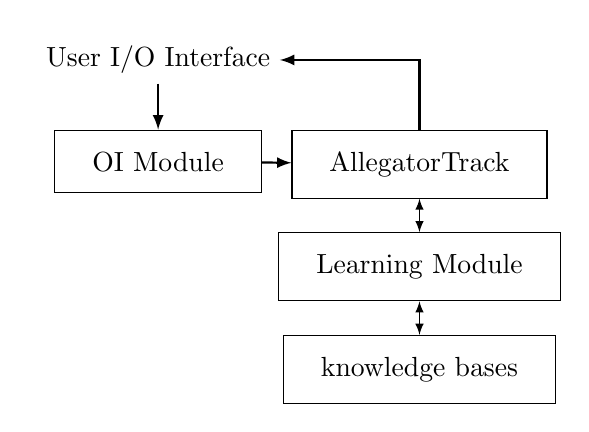
\begin{tikzpicture}[auto, line/.style ={draw,  thick, shorten <=0pt}]
  \matrix[matrix of nodes, row sep=5ex, column sep=1em] (mx) {
    User I/O Interface &\\
    OI Module &  AllegatorTrack\\
    & Learning Module\\ 
    & knowledge bases \\
  };
  %\node[ou=(mx-1-3)] (empty) {};
  \node[ou=(mx-2-1)] (oi) {};
  \node[ou=(mx-2-2)] (tf) {};
  \node[ou=(mx-3-2)] (lm) {};
  \node[ou=(mx-4-2)] (kb) {};
  %{[->, thick]
  %\draw(mx-1-1)edge(empty);
  %}
  {[->, thick]
  \draw(mx-1-1)edge(oi);
  \draw(oi)edge(tf);
  }
  {[<->]
    \draw(tf)edge(lm);
     \draw(lm)edge(kb);
  }
  \begin{scope}[every path/.style=line, <-]
   \path(mx-1-1)  - | (tf);
  % \path(mx-1-3)  - | (lm);
  \end{scope}

\end{tikzpicture}
\caption{Architecture of our system}\label{system_architecture}
\end{figure}
% Demonstration scenario
\subsection{Demonstration Scenario}
A given user that wants to interact with our system
must do it through the search form. Through the search
form, she (or he) provides her searched relation, e.g.,
\textquote{Where is born Barack Obama?}. The searched relation is then 
passed to the information extraction engine,  TextRunner system
in our case, which returns a set of answers considered to be 
relevant for the user's request. Each claim in the returned list is
processed in order to extract the corresponding sources along a detailed
description of the claim which we format in a certain manner. The 
set of sources and the formatted versions of all claims are then passed
to the truth finding module which integrate all the claims and compute the
most probable answer together with the reliability scores of participated 
sources for the searched relation. Finally, the output of the truth finding
process is returned to the user. The user can also want to review the output
of our system by definitively validiting it or not through its knwoledge of the
modeled world. For example when the system has totally wrong, it may be interesting
to get such a kind of feedbacks from the user in order to change the used method, as
there are many available with our system, and to enhance the process for the further 
search about the same world. The user gives feedbacks using the option buttons on the 
left-hand side of the outputted claims or the text form. The feebacks given by the user
is saved in knwoledge bases within our system for further processes.

% Conclusion
\section{Conclusion}
% References
\cite{*}
\bibliographystyle{plain}
\bibliography{biblio}

\end{document}
